
\chapter{Introduction}


\section{Problem Background}
\label{sec:chap1-problem}

%- what is the permian basin
%- why important
%- why people care about it
%- roger spent lots of time to convince why it's hard (complicated cross section structures). it's nothing to do with his work! but you show you really understand the problem and wha you're working with
%- the most important before contribution is to try to illustrate why it's a hard problem
%- not only we focused on techcnial, and work on problem that matters, but dont forget why **insar over west texas is hard**


%- first paragraph: convince it's super important problem. why perimain basin matters, and what's the problem
%- have wells, inducsed seismicity, rate hasskyrocket, mention one year has more than CA.
%- also btw, this is difficult. not all wells induce. some wells opearate fine, no issues, some wells have delayed, and keep having EQs about stop.
%- even people without background should find intersting, even without texas background.
%- people in general like to hear problems, and where people are stuck, and why they care to work on.
%- Natl academy science report shold have highlights to take.
%- ESI proposal: use from that

The Permian Basin, stretching from eastern New Mexico and covering most of West Texas (Figure \ref{fig:permian-overview}a), has become the United States' largest producer of oil and gas over the past decade. The region's production began to take off in the late 2000s, largely due to advances in horizontal drilling and multi-stage hydraulic fracturing.
Since that time, the basin also experienced an increased rate of low magnitude earthquakes \citep{Frohlich2016HistoricalReviewInduced, Atkinson2016HydraulicFracturingSeismicity, Frohlich2019OnsetCauseIncreased, Lomax2019ImprovingAbsoluteEarthquake, Savvaidis2020InducedSeismicityDelaware, Skoumal2020InducedSeismicityDelaware} (Figure \ref{fig:permian-overview}b).


Since the 1920s, researchers have recognized that injection or withdrawal of fluids from the subsurface can induce earthquakes along existing faults \citep{Council2013InducedSeismicityPotential, Simpson1988TwoTypesReservoir, Ellsworth2013InjectionInducedEarthquakes}.  Induced earthquakes near oil production and wastewater injection wells have been recently observed in the central and eastern United States in Arkansas, Ohio, Oklahoma, Texas, as well as other countries including Canada, China, and Italy \citep{Foulger2018GlobalReviewHuman}.  In Texas, despite rising volumes of production and wastewater injection throughout the Permian Basin, the recently cataloged earthquakes are spatially clustered. The vast majority of production and injection wells experience no nearby seismic activity; however, the earthquake clusters within Texas contained over 200 earthquakes of magnitude 3.0 or greater in 2021, second only to California in the contiguous United States.


\begin{figure}
	\centering
	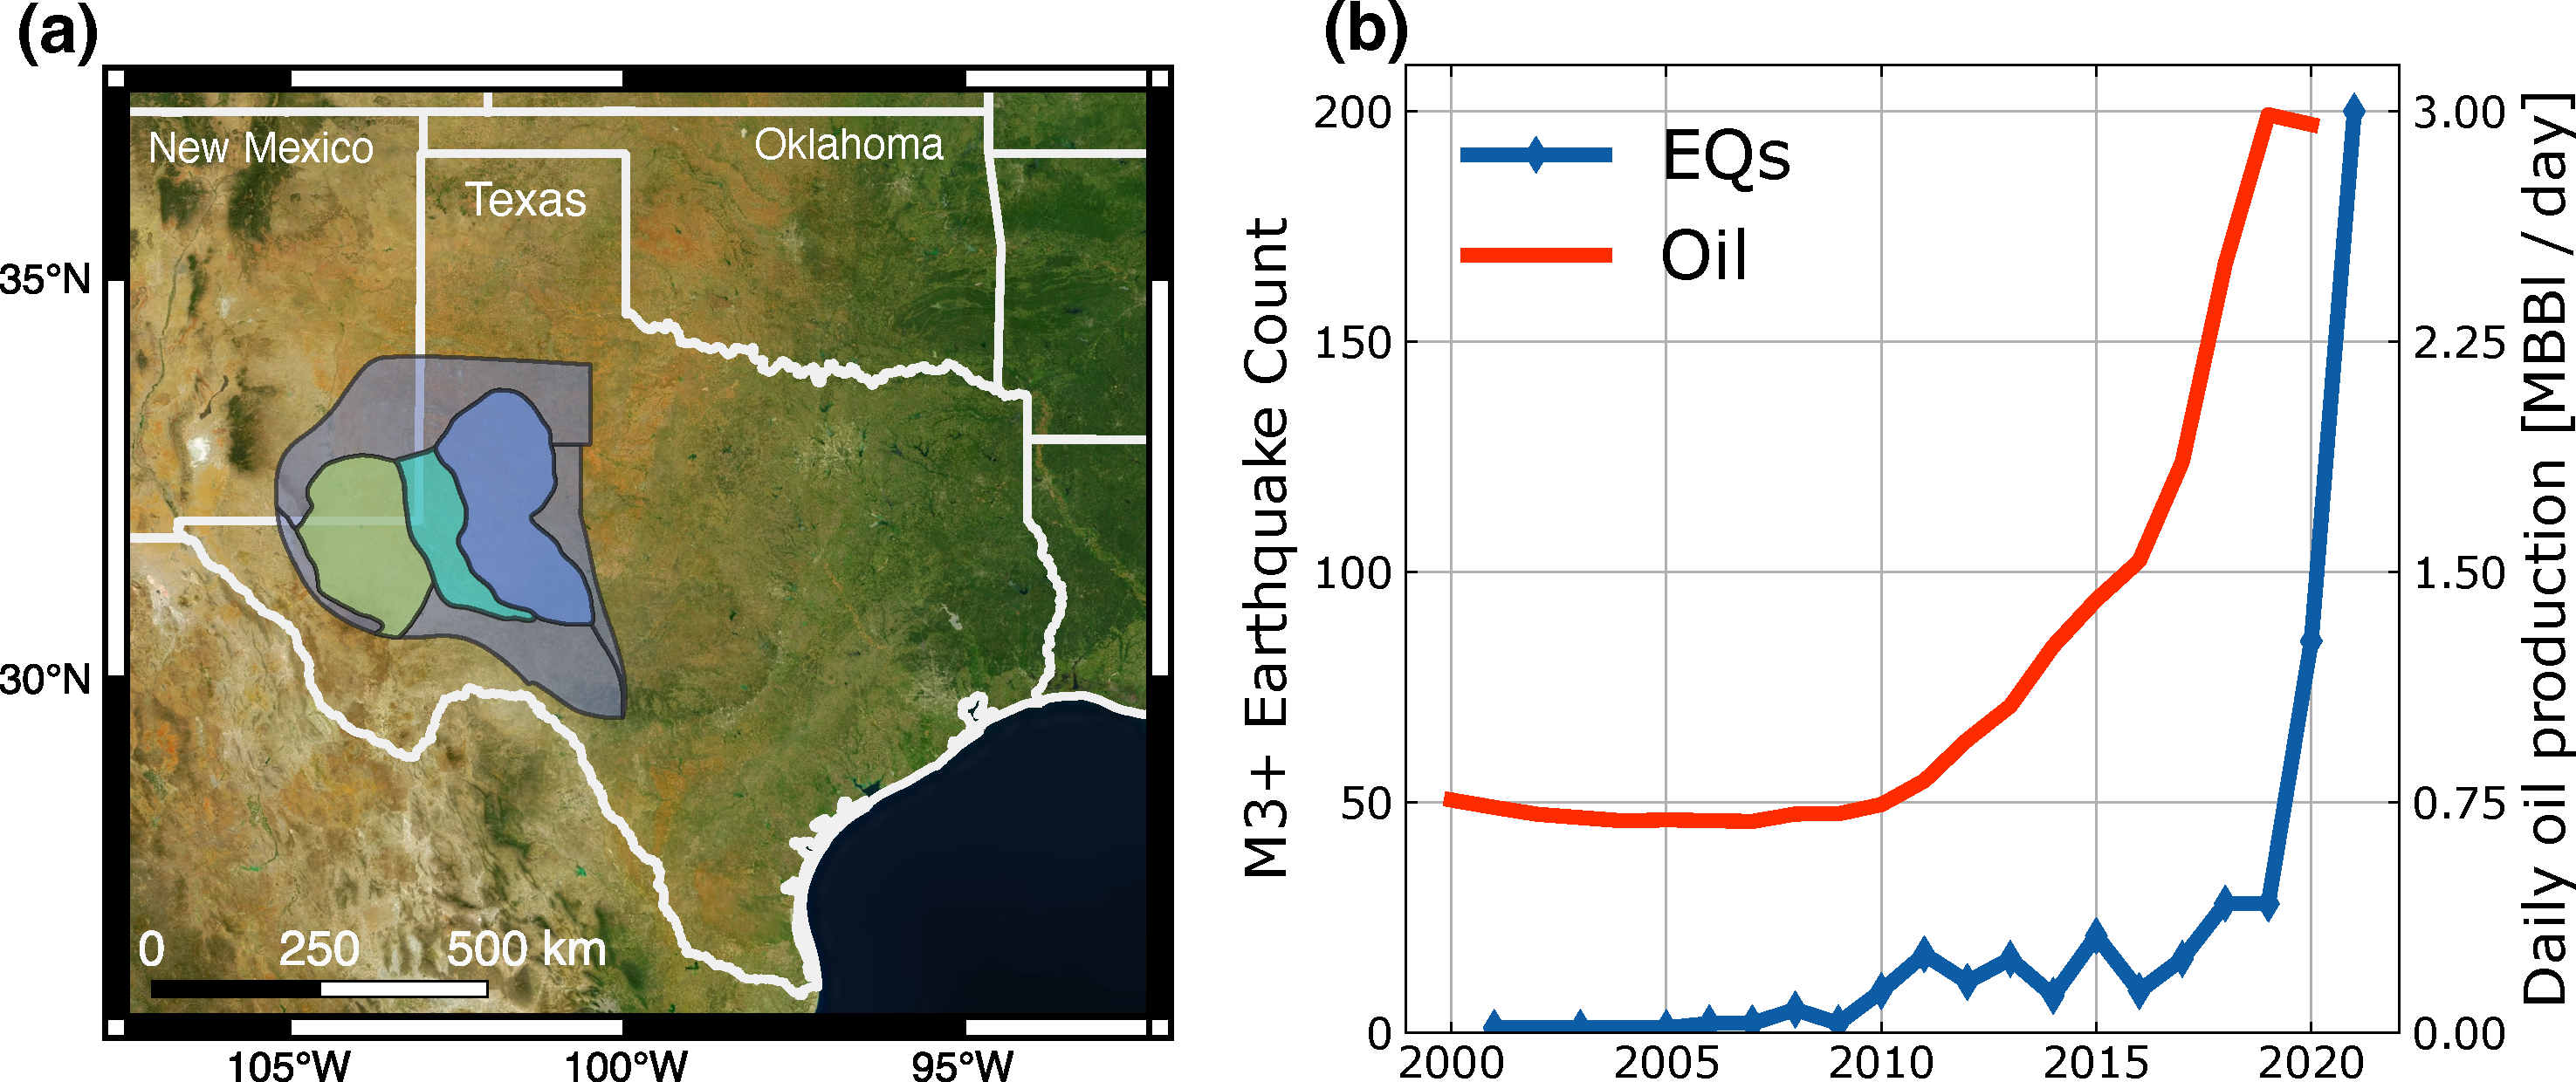
\includegraphics[width=\columnwidth]{figures/permian-overview-eqs-oil.pdf}
	\caption[Permian Basin oil production and earthquakes]{
		(a) Location of Permian Basin within Texas. The subbasins colored within the Permian Basin are (from west to east) the Delaware Basin (green), Central Basin Platform (cyan), and Midland Basin (purple).
		(b) Yearly number of magnitude 3 or larger earthquakes recorded within Texas since 2000 (blue line), and average daily oil production per year for Permian Basin wells in Texas (red line).
		Earthquakes retrieved from USGS at \url{https://earthquake.usgs.gov} . Oil Production data retrieved from the Texas Railroad Commission's production query system at \url{https://www.rrc.texas.gov} .
	}
	\label{fig:permian-overview}
\end{figure}



%One significant cluster is near Pecos, TX, where increased seismic activity began in 2009 and climbed to more than 2000 earthquakes in 2017 \citep{Frohlich2019OnsetCauseIncreased}. 

Understanding the causes of induced earthquakes be challenging, as there is limited knowledge of the locations of subsurface faults and the ways in which petroleum operations affect pore pressure \citep{Hennings2021StabilityFaultSystems}. Additionally, the Permian Basin contains many possible mechanisms which can trigger earthquakes, including oil and gas production, wastewater injection, hydraulic fracturing, and groundwater withdrawal, all operating in a geologically-complex region \citep{Smye2021VariationsVerticalStress}.
Although detailed measurement of the subsurface is infeasible across the $\sim$200,000 km$^2$ Permian Basin, the spaceborne remote sensing technique known as Interferometric Synthetic Aperture Radar (InSAR) can measure deformation of Earth's surface over wide areas with millimeter-to-centimeter accuracy \citep{Massonnet1993DisplacementFieldLanders, Buergmann2000SyntheticApertureRadar}. These surface deformation measurements can be used to derive information about Earth's subsurface, locate previously unknown faults, estimate the distribution of fault slip, and infer associated seismic risk \citep{Segall2010EarthquakeVolcanoDeformation, Elliott2016RoleSpaceBased, Huang2017FaultGeometryInversion}.

Previous InSAR studies over West Texas demonstrated the use of InSAR surface deformation data for understanding causes of induced seismicity.
For example, \cite{Kim2018AssociationLocalizedGeohazards} detected multiple deformation bowls within the Delaware Basin related to wastewater injection, $CO_2$ injection, and hydrocarbon production using Sentinel-1 InSAR data. \cite{Deng2020SurfaceDeformationInduced} used ascending Sentinel-1 LOS measurements to infer pore pressure change and Coulomb failure stress change at three sites in the southern Delaware Basin. 
However, these studies only focused on study areas $ \sim $ 60$ \times $60km or smaller. Since InSAR noise becomes more severe as the area of interest expands, it is difficult to cover to the entire Permian basin while retaining millimeter level accuracy. 

Additionally, the volume of available InSAR data has grown exponentially since the launch of Sentinel-1 in 2014. This expansion has prompted the need to develop automated methods of detecting deformation sources in large surface deformation maps.
Previous studies have applied computer vision and machine learning techniques for automated detection \citep{Anantrasirichai2018ApplicationMachineLearning, RouetLeduc2021AutonomousExtractionMillimeter, Ebmeier2016ApplicationIndependentComponent}; however, residual InSAR noise can often visually be mistaken for real deformation.
While auxiliary data sources can be used to quantify uncertainty in deformation maps \citep{Barnhart2013CharacterizingEstimatingNoise, Parker2015SystematicAssessmentAtmospheric}, these measurements typically do not have sufficient resolution to capture the kilometer-scale noise which regularly appears due to West Texas summer weather patterns.

%Since uncertainty quantification based on auxiliary measurements typically do not have sufficient resolution 
%the associated uncertainty quantification has usually been derived from auxiliary data sources. Since these data sources typically do not have sufficient spatial resolution to capture spatially coherent noise, 




%However, InSAR measurements contain many noise sources which pose serious challenges for attempts at routine processing over large areas.
%Specifically, errors from atmospheric noise can be over 10x as large as the deformation signals of interest.
%While InSAR has the possibility of providing a key observable for basin-scale studies on induced seismicity and its mitigation, it is necessary to mitigate the severe noise and provide detailed uncertainty measures to stakeholders.


%%%%%%%%%%%%%%%%%%%%%%%%
%Within Texas, \cite{Shirzaei2016SurfaceUpliftTime} reported indications of surface uplift due to wastewater injection near a 2012 M4.8 earthquake, though limited validation for the ALOS data was available at this site near Timpson, TX \citep{Semple2017IncompleteInventorySuspected}. \cite{Kim2018AssociationLocalizedGeohazards} detected multiple deformation bowls within the Delaware Basin related to wastewater injection, $CO_2$ injection, and hydrocarbon production using Sentinel-1 InSAR data. \cite{Zheng2019WastewaterLeakageWest} incorporated InSAR-derived surface deformation data into a poroelastic model to analyze the geomechanical processes near an uplift signal in northern West Texas. They discovered that the observed surface deformation was likely caused by injection well leakages, rather than pressure increases at the planned injection depth, and the leaks may have contributed to freshwater contamination. More recently, \cite{Deng2020SurfaceDeformationInduced} used ascending Sentinel-1 LOS measurements to infer pore pressure change and Coulomb failure stress change at three sites in the southern Delaware Basin. They suggested that certain groups of earthquakes are likely induced by fluid injection, but noted that local rock structure and media properties are key controls on the area's susceptibility to induced seismicity.

%Previous InSAR studies demonstrated the use of InSAR surface deformation data for understanding causes of induced seismicity; however, these studies only focused on study areas $ \sim $ 60-by-60km or smaller, and basin-wide InSAR surface deformation data with detailed uncertainty quantification are needed for assessing the likelihood of induced seismicity risk. Since InSAR tropospheric noise variance increases with the distance away from the reference point \citep{Emardson2003NeutralAtmosphericDelay}, it is difficult to expand the InSAR spatial coverage to the entire Permian basin while retaining millimeter level accuracy. 

%%%%%%%%%% TGRS %%%%%%%%%%%%
%Interferometric Synthetic Aperture Radar (InSAR) has made it possible to monitor surface deformation with 10s–100s meter spatial resolution and millimeter-to-centimeter accuracy (e.g. \citep{Pritchard2004InSARbasedsurvey,  Chaussard2014PredictabilityHydraulicHead,  Chen20142010SlowSlip, Biggs2017GlobalVolcanoMonitoring, Chen2016ConfinedAquiferHead, Fielding2017SurfaceDeformationNorth, Chen2019TriggeringMw7.2}). Since the launch of the Sentinel-1 mission in 2014, the quantity and quality of open-access InSAR data has grown exponentially. Processing and interpreting such data often requires artificial intelligence and computer vision algorithms without extensive manual inspection. However, designing robust and scalable computer vision algorithms for automatic detection of InSAR surface deformation features is challenging. This is because InSAR measurement noise varies substantially in both space and time, and its magnitude is often comparable or larger than subtle deformation signals of interest. In particular, residual troposphere noise in InSAR surface deformation maps are spatially coherent, and it can often be visually mistaken as real surface deformation.


%To address these challenges, previous studies developed algorithms for detecting deformation signals in pixel-wise InSAR deformation time series based on certain magnitude thresholds. The thresholds can be set manually \citep{Raspini2018ContinuousSemiAutomatic}, set using pixel-wise standard deviations \citep{Bekaert2020InsarBasedDetection}, derived from auxiliary data sources (e.g. global atmospheric weather models \citep{Parker2015SystematicAssessmentAtmospheric}, MODIS water vapor measurements \citep{Barnhart2013CharacterizingEstimatingNoise}), or derived from simulated noise parameters \citep{Havazli2021DetectionThresholdEstimates}. Principal component analysis (PCA) and independent component analysis (ICA) have also been used to explore decompositions of noisy time series data \citep{Chaussard2014PredictabilityHydraulicHead, Ebmeier2016ApplicationIndependentComponent, Gaddes2018BlindSignalSeparation}. Moreover, deep learning methods using convolutional neural networks (CNNs) have been applied to detect deformation features in individual interferograms \citep{Anantrasirichai2018ApplicationMachineLearning, Anantrasirichai2019ApplicationConvolutionalNeural} or InSAR time series \citep{RouetLeduc2021AutonomousExtractionMillimeter}. Because the detection problems are posed as a supervised learning task, they require either labeled training data \citep{Anantrasirichai2018ApplicationMachineLearning} or ground truth examples from simulated noise and deformation models \citep{Anantrasirichai2019DeepLearningApproach, RouetLeduc2021AutonomousExtractionMillimeter}. These supervised learning approaches work well when deformation signals of interest show spatial signatures that are distinct from InSAR measurement noise. In many applications, both deformation signals and tropospheric turbulence noise are spatially coherent ``blob-like'' features that look similar to human eyes.

%Automatic detection algorithms need to quantify the detection uncertainty based on the noise magnitude of a particular radar dataset. Auxiliary tropospheric data sources such as MODIS or weather models typically do not have sufficient spatial resolution to capture localized tropospheric turbulence noise at sub-kilometer scale. Here we present


\section{Contributions}
\label{sec:chap1-contributions}


The contributions of this thesis center around designing scalable methods to produce reliable surface deformation maps over large regions. We have focused on the mitigation of strong atmospheric noise and the creation of uncertainty measures which are easy to interpret for non-expert stakeholders.


The contributions may be summarized as follows:

\begin{enumerate}
	
	\item We developed Python-based InSAR time series analysis software to ingest geocoded SAR images, extract surface deformation, decompose multiple geometries into horizontal and vertical deformation, and verify results with permanent GPS stations.
	
	\item We performed a rigorous uncertainty analysis to identify the dominant noise source in the Permian Basin for Sentinel-1.  In the process, we developed a method to estimate the tropospheric noise and its power spectral density from InSAR data.
	
	\item We designed scalable, robust time series algorithms for tracking yearly changes of deformation over large regions.
	
	\item We created millimeter-level accurate maps of cumulative surface deformation that are available online for analysis. These maps contain many subsidence and uplift features near oil and gas production, as well as linear patterns near clusters of seismic activity.
	
	\item We created a computer vision algorithm to automatically detect surface deformation signals of unknown sizes in large InSAR maps. The detection algorithm produces uncertainty estimates for each visual feature in the InSAR data.
	
	
	
\end{enumerate}


\section{Thesis Roadmap}
\label{sec:chap1-roadmap}


In Chapter \ref{CHAP:2}, we introduce the principles of InSAR. We start with a review of synthetic aperture radar (SAR) image formation. We show how the phase difference between two SAR images acquired at different times can be used to infer topography or surface deformation. We outline common InSAR noise sources, emphasizing the origins of tropospheric noise, and how to combine many interferograms to solve for a time series of surface deformation. We show how the use of geocoded single-look complex (SLC) products enables a simple InSAR processing workflow. Finally, we describe how to decompose deformation from multiple satellite geometries into horizontal and vertical components.


In Chapter \ref{CHAP:3}, we introduce the scientific background of the induced seismicity problem. We review the oil and gas production boom of the last decade within the Permian Basin, as well as previous studies on the increase in low magnitude earthquakes during this time. We describe the geodetic datasets available to study the problem, and we present the case to use InSAR 
%for new high-quality observational datasets 
to better inform efforts to mitigate induced seismicity.


In Chapter \ref{CHAP:4-GRL}, we present a simple yet effective time series method for creating cumulative surface deformation maps over large regions with severe tropospheric noise. We use the method to create yearly deformation maps over the oil-producing region of the Permian Basin. The method incorporates an automated outlier detection and removal algorithm, which enabled ~2 mm/year agreement with GPS measurements in the presence of $\sim$15 cm of tropospheric noise.


In Chapter \ref{CHAP:5-robust-ts}, we expand our robust time series methods to account for non-linear deformation. We introduce a method to extract nonlinear deformation over long time series using non-parametric LOWESS smoothing. We demonstrate the method's ability to mitigate strong tropospheric noise on synthetic data. We use the method on Sentinel-1 data to create yearly cumulative and differential surface deformation maps for 2015-2021 over the Permian Basin, where a variety of anthropogenic causes have led to local and large-scale deformation patterns.


In Chapter \ref{CHAP:6-blob}, we demonstrate methods for automatically detecting surface deformation signals in InSAR maps. We present a computer vision algorithm based on Laplacian of Gaussian filters. We show how the tropospheric noise levels can be estimated from InSAR data, and we use these estimates to simulate new instances of noise. We create confidence measures based on the simulations for automatically detected signals in real InSAR maps.


Finally, we conclude in Chapter \ref{CHAP:7} with a summary and discussions of possible directions of future research.
